\documentclass[11pt,a4paper]{article}

\usepackage[english]{babel}
\usepackage[T1]{fontenc}
\usepackage[utf8]{inputenc}
\usepackage{graphicx}
\graphicspath{{../Figs/}}
\usepackage{float}
\usepackage{subcaption}
\usepackage[font=footnotesize,labelfont={sf,bf},textfont=sf,width=\textwidth]{caption}
\usepackage[margin=2cm]{geometry}
\usepackage[plainpages=false,pdfpagelabels,hypertexnames=false]{hyperref}
\usepackage[usenames,dvipsnames]{xcolor}
\usepackage{mathtools}
\usepackage[separate-uncertainty=true]{siunitx}
\usepackage{booktabs}
\usepackage[title]{appendix}

\title{\bfseries\textsc{Atomic Force Microscopy}}
\author{
Michele Masini\\ \small\texttt{\href{mailto:michele.masini@uni-ulm.de}{michele.masini@uni-ulm.de}}\and
Iyán Méndez Veiga\\ \small\texttt{\href{mailto:iyan.mendez-veiga@uni-ulm.de}{iyan.mendez-veiga@uni-ulm.de}}
}
\date{\today}


\begin{document}
\maketitle

\begin{abstract}
Atomic Force Microscopy (AFM) is not common in bachelor laboratories. Our motivation for doing this experiment was to understand the theory of AFM and to use one of these devices for the first time. We measured a calibration grid and three different samples using the \href{https://www.nanosurf.com/en/products/naioafm-the-leading-compact-afm}{NaioAFM} by Nanosurf company in static and tapping mode.

We found working in the tapping mode easier, perhaps due to an inappropriate tip for the static mode. Not relevant differences were noticed for setpoints between \SI{2}{\nano\N} and \SI{20}{\nano\N} in static mode but an upper limit of 65\% in the tapping mode was found. Significantly larger height values than those provided by the calibration sample were measured.  In tapping mode, I-Gain was the most relevant PID value after optimizing the setpoint. Interesting patterns were found in two of the samples and there were characterized by measuring the height and separation distance of the features.
\end{abstract}

\section{Introduction}

Since it was first developed in 1985 by \emph{Binning} et al., the Atomic Force Microscopy (AFM) \cite{Bhushan} has become a popular surface profiler for topographic and normal force measurements on the micro- to nanoscale. Not only AFMs, but also modified devices such as Lateral Force Microscopies (LFMs) or Friction Force Microscopies (FFMs), have found applications in different fields.

In this report, we will first describe the AFM technique, the two different operation modes that we used (static and tapping mode) and comment the issues we faced, as well as a general overview of the relevant AFM image artifacts for us, i.e., features which appear in the images that are not present in the original probed object. Then, we will describe the processing of raw data obtained from the device using the open source software Gwyddion, compare the obtained results with the theoretical ones for a calibration sample, and show the obtained images for the three different samples.

\subsection{Theory of AFM}

AFM is quite similar to Scanning Tunneling Microscope (STM). The idea is to get 3D images of sample surfaces by using a scanning technique. The main difference between AFM and STM is that AFM can also measure insulators and it is not limited to conductors because the scanning technique does not make use of tunneling currents. Instead, AFM is able to obtain the height by measuring the ultrasmall forces that arise when the tip and the sample surface get very close to each other. The order of magnitude of these forces is less than \SI{1}{\nano\N}.

A fixed relation between these forces and the distance between the tip and the sample allows to get the profile of the surface. However, this depends on the operation mode.

\begin{figure}[ht]
\centering
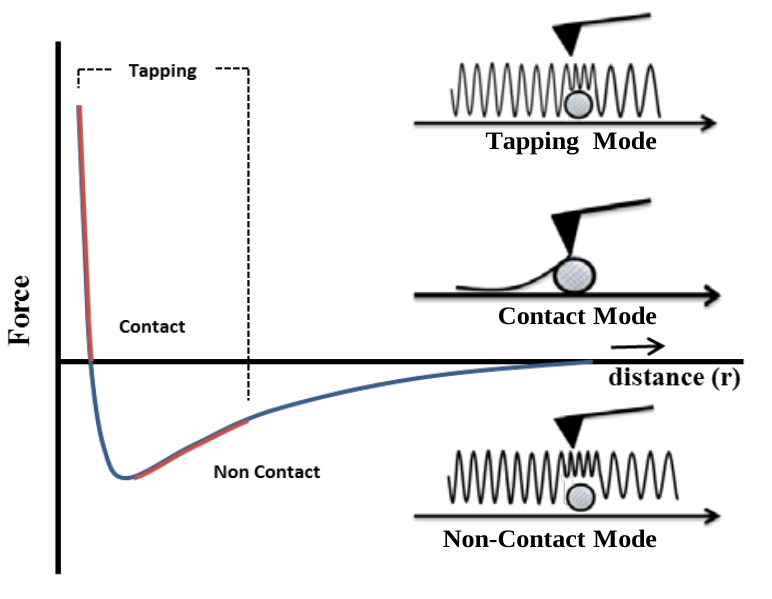
\includegraphics[width=0.7\textwidth]{AFM_modes}
\caption{Force that the tip experiments against the distance with respect to the surface of the sample \cite{jfb8010007}. In the contact mode forces are repulsive while in the non conntact mode are attractive. In the dynamic or tapping mode we are in between but typically closer to the repulsive barrier.}
\label{fig:AFM_modes}
\end{figure}

Basically, we can say that AFM can be used in two main modes or regimes: static, repulsive or contact mode, and dynamic or tapping mode. The curve for the force that the tip feels at different distances (Figure \ref{fig:AFM_modes}) can be model using the Lennard-Jones potential:

\begin{equation}\label{eq:LJ}
V(r)=V_0\left[\left(\frac{r_0}{r}\right)^{12}-2\left(\frac{r_0}{r}\right)^6\right]\,,
\end{equation}
which has a repulsive term ($\sim1/r^{12}$) and an attractive one $(\sim1/r^6$). $V_0$ is the depth of the potential well and $r_0$ is the distance at which $V'(r)=0$.

The most fragile part of the AFM, and at the same time one of the most important parts in order to do good measurements is the cantilever, where a sharp tip is placed almost at one of its ends. The cantilever has to be very flexible in the normal direction so it can deflect depending on the force that the tip "feels". In the static mode, the tip is in contact with the surface of the sample and it is repulsed by it due to the electronic overlap between the atoms of the tip and the ones in the sample ($1/r^{12}$ term in the Lennard-Jones potential from eq.~\eqref{eq:LJ}). If the cantilever spring constant is known, then by measuring its deflection we can obtain the forces. There are many methods to measure this deflection such as using tunneling, capacitive or optical detectors with lasers (see Figure \ref{fig:Deflection_measurement}).

\begin{figure}[ht]
\centering
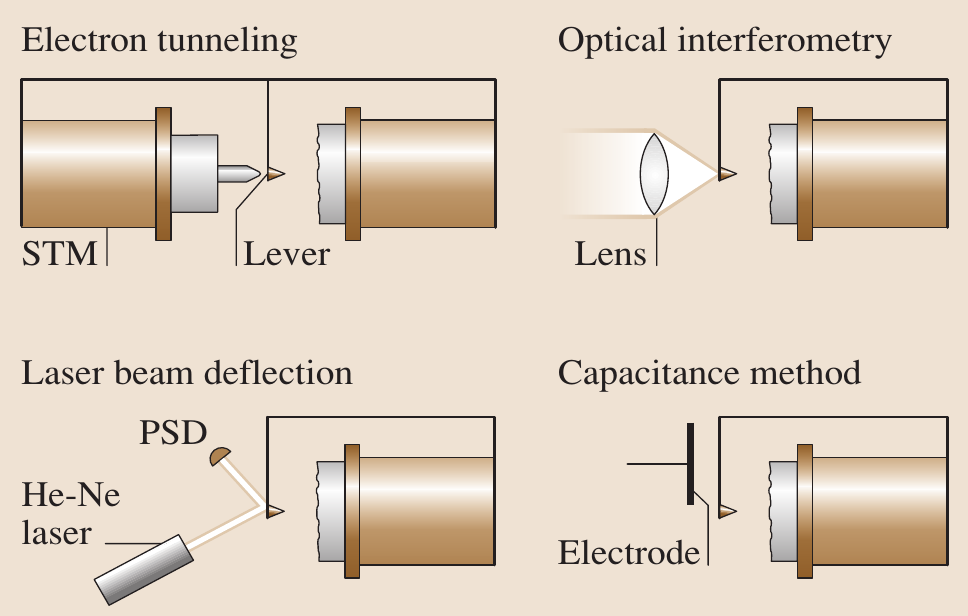
\includegraphics[width=0.5\textwidth]{Deflection}
\caption{Different techniques to measure cantilever deflection in an AFM \cite{Bhushan}.}
\label{fig:Deflection_measurement}
\end{figure}

The deflection can be measured to within \SI{0.02}{\nm}, so for a typical cantilever spring constant of \SI{10}{\N/\m}, forces as low as \SI{0.2}{\nano\N} can be measured.

However, it is not usual to measure the height of the sample directly from the deflection. Typically, this signal is used as the input for a feedback mechanism. Whenever there is a change in the force affecting the tip, and therefore a change in the deflection, the distance $r$ between the tip and the sample will be move accordingly to keep this deflection constant. This is achieved using piezo materials and the force that keeps the desired deflection of the cantilever is called \emph{setpoint}. Moreover, in order to get a profile of the whole surface, either the tip or the sample has to be translated. More details about the feedback mechanism can be read in section \ref{sec:feedback}.

When we are on the right of the equilibrium (Figure \ref{fig:AFM_modes}), the attractive forces on the tip are very weak van der Waals forces ($1/r^6$ term in the Lennard-Jones potential eq.~\eqref{eq:LJ}). Tapping mode can be used on this regime and the main difference is that we do not measure the force anymore, but the force gradient. The cantilever is deliberately vibrated at its resonant frequency $\omega_0$ given by the spring constant and the force derivative is determined by measuring the shift in this resonant frequency due to the interaction with the sample. Tapping mode can used either in amplitude (AM) or frequency modulation (FM).

\begin{figure}[ht]
\centering
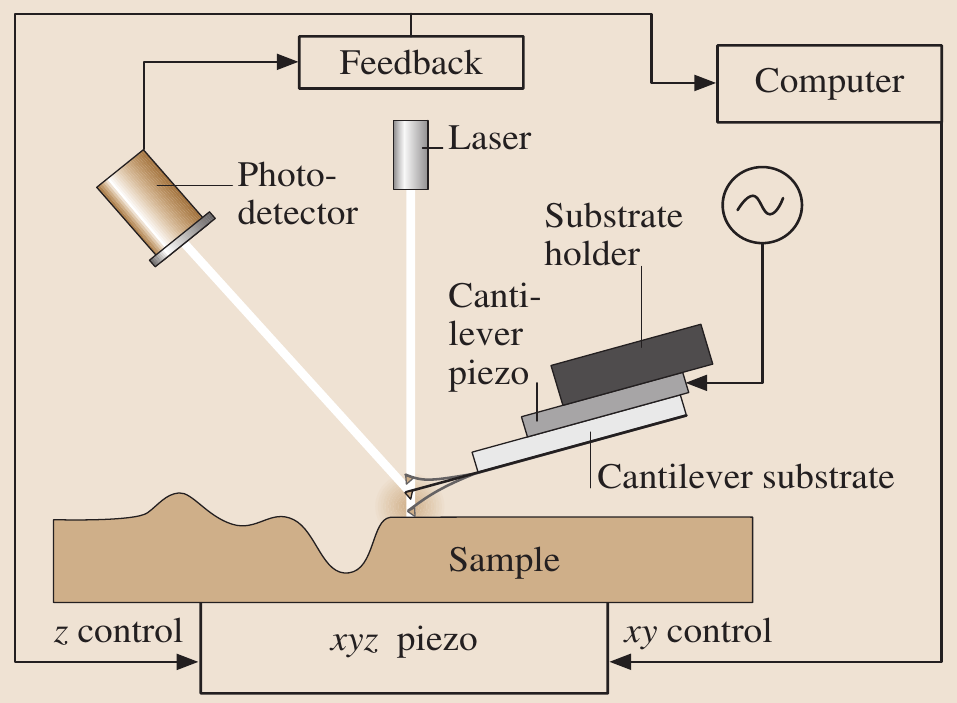
\includegraphics[width=0.5\textwidth]{Tapping_mode}
\caption{Schematic of tapping mode using a feedback mechanism to keep resonant frequency $\omega_0$ of the cantilever constant \cite{Bhushan}.}
\label{fig:measurement_tapping}
\end{figure}

Similarly to the static mode, we can directly measure the force gradient or we can use it as a signal for a feedback mechanism that acts on the distance $r$ to keep the resonant frequency constant. An schematic draw is shown in Figure \ref{fig:measurement_tapping}.

\subsection{Feedback mechanism}\label{sec:feedback}
We have mentioned in the previous section that the AFM can be used with or without a feedback mechanism, but since in the experiment we used it both for static and tapping modes, we will describe this technique very briefly.

Feedback mechanisms and feedback parameters are ubiquitous in our life \cite{nanosurf}. For example, when we use a thermostat, the temperature is the feedback parameter, which is set to a a desired one (\emph{setpoint}) and as the temperature in the room changes, it is compared with the temperature setpoint so that a feedback mechanism (e.g. an air conditioner) can act to keep the temperature at the desired value. Mathematically, all these mechanisms are applications of the control theory developed during the 19th century.

\begin{figure}[hbt]
\centering
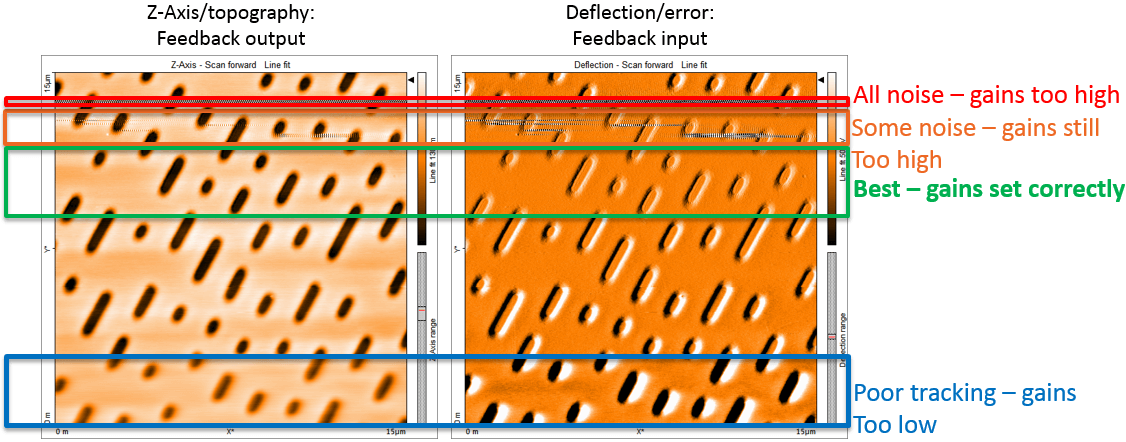
\includegraphics[width=0.8\textwidth]{afm-modes-feedback}
\caption{Feedback input and output signals for different values of PID gains \cite{nanosurf}.}
\label{fig:feedback}
\end{figure}

The feedback parameter that serves as the setpoint in contact mode is the the cantilever deflection. In the tapping mode, it is the cantilever oscillation amplitude.

The feedback mechanism is a continuous loop, the so-called feedback loop, which is controlled through the proportion-integral-derivative control, also referred as the PID gains. These different gains refer to differences in how the feedback loop adjusts to deviations from the setpoint value, i.e. the error signal. 

If gains are set too low, the PID loop is not able to keep the setpoint accurately. Contrary, if gains are chosen too high, the result will be electrical noise in the image interference from the feedback (see Figure \ref{fig:feedback}). This is due to the fact that compensation for a deviation from the setpoint is larger than the error itself.

Nevertheless, gains are not the only parameters that affect the feedback mechanism. The scan rate and, of course, the setpoint value are very important, too. If the scan rate is too fast, the PID loop will not have sufficient time to adjust the feedback parameter to its setpoint value and the height calculated from the z-piezo movement will deviate from the true topography at slopes and near edges. Very slow rates do not affect the quality of the obtained topography since they are not an issue for the PID loop, but they lead to long acquisition times.

Optimization of both scan rate and PID gains are necessary in order to optimize the feedback loop.

\subsection{AFM artifacts}
When using an AFM, as well as in many other experiments, we may find features which appear in the obtained images that are not present in the observed sample. These are called artifacts \cite{artifacts} and there are four primary sources of artifacts in images measured with AFMs: probes, scanners, image processing and vibrations.

\begin{figure}[ht]
\centering
\begin{subfigure}[b]{0.45\textwidth}
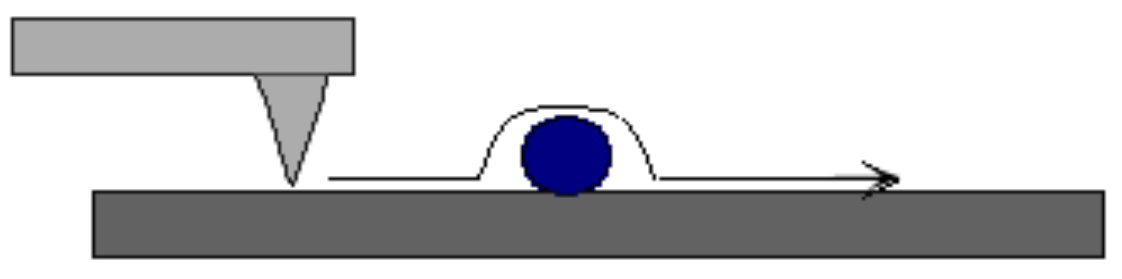
\includegraphics[width=\textwidth]{artifacts_probe_1}
\caption{Feature appears too large}
\label{fig:artifacts_probe_1}
\end{subfigure}
\begin{subfigure}[b]{0.45\textwidth}
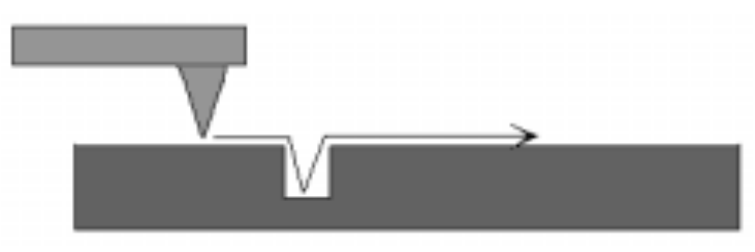
\includegraphics[width=\textwidth]{artifacts_probe_2}
\caption{Feature appears too small}
\label{fig:artifacts_probe_2}
\end{subfigure}\\\vspace{.2cm}
\begin{subfigure}[b]{0.45\textwidth}
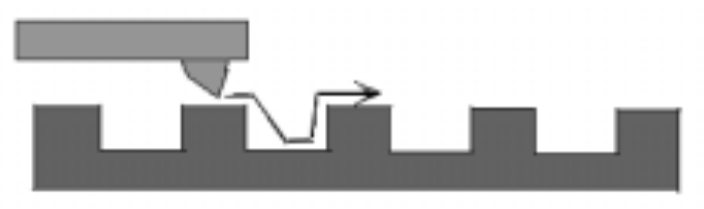
\includegraphics[width=\textwidth]{artifacts_probe_3}
\caption{Distorsion caused by a chipped tip}
\label{fig:artifacts_probe_3}
\end{subfigure}
\caption{Some examples of probe-generated artifacts \cite{artifacts}.}
\label{fig:artifacts_probe}
\end{figure}

Images measured with an AFM are always a convolution of the probe geometry and the shape of the features being imaged. In order to avoid probe-generated artifacts, the tip should be much smaller than the features being measured. When this condition is not satisfied or if the tip is damaged, features on the sample may appear larger, smaller or with strangely shaped patterns as shown in Figure \ref{fig:artifacts_probe}.

Artifacts may also arise due to the motion of the scanner in the X, Y and Z directions. Piezoelectric materials move in a nonlinear motion when a linear voltage ramp is applied. If they are not well calibrated, sizes and forms my appear severely distorted (see Figure \ref{fig:artifacts_scanner_1}). Besides, the geometry of the scanner and the positioning of it relative to the sample can also create artifacts (see Figure \ref{fig:artifacts_scanner_2}).

\begin{figure}[H]
\centering
\begin{subfigure}[b]{0.45\textwidth}
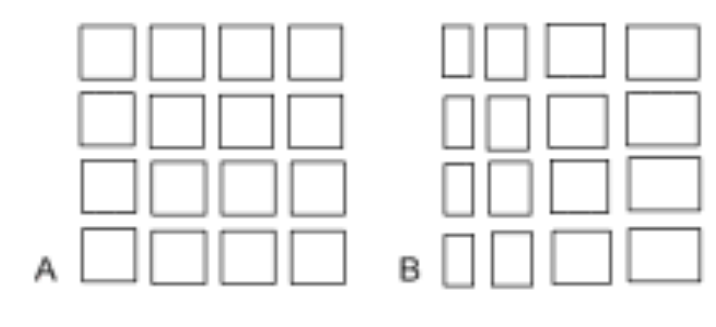
\includegraphics[width=\textwidth]{artifacts_scanner_1}
\caption{A test pattern with squares (left) distorted in the AFM (right) due to nonlinearity of the piezo materials}
\label{fig:artifacts_scanner_1}
\end{subfigure}
\begin{subfigure}[b]{0.45\textwidth}
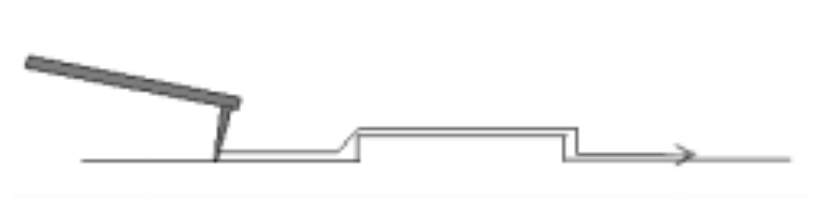
\includegraphics[width=\textwidth]{artifacts_scanner_2}
\caption{Artifact due to the probe sample angle}
\label{fig:artifacts_scanner_2}
\end{subfigure}
\caption{Some examples of scanner-generated artifacts \cite{artifacts}.}
\label{fig:artifacts_scanner}
\end{figure}

Processing images is a must when dealing with AFM, but additional artifacts can be introduced if the processing software is not properly used. For example, bands that do not correspond to a real structure may appear when subtracting the background (see Figure \ref{fig:artifacts_processing}).

\begin{figure}[H]
\centering
\begin{subfigure}[b]{0.3\textwidth}
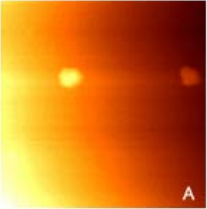
\includegraphics[width=\textwidth]{artifacts_processing_1}
\caption{Image obtained from AFM before any processing}
\label{fig:artifacts_processing_1}
\end{subfigure}
\begin{subfigure}[b]{0.3\textwidth}
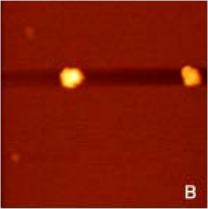
\includegraphics[width=\textwidth]{artifacts_processing_2}
\caption{After a line-by-line leveling with a background correction}
\label{fig:artifacts_processing_2}
\end{subfigure}
\begin{subfigure}[b]{0.3\textwidth}
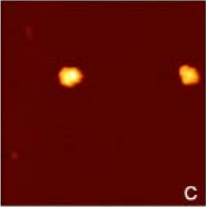
\includegraphics[width=\textwidth]{artifacts_processing_3}
\caption{Particles excluded from the background subtraction}
\label{fig:artifacts_processing_3}
\end{subfigure}
\caption{Some examples of processing-generated artifacts \cite{artifacts}.}
\label{fig:artifacts_processing}
\end{figure}

Of course, there are many other artifacts but these are the most relevant for our experimental setup with the NaioAFM.

\section{Materials and methods}

\subsection{NaioAFM}

The NaioAFM by Nanosurf \cite{NaioAFM} is the AFM used in this experiment. As the successor of the Easyscan 2, the NaioAFM is a compact AFM designed for new and inexperienced AFM users. It has a closed scanner compartment that helps with acoustic and air current isolation, and stage positioners to adjust the sample without having to open the compartment. The different parts of the scan head including the spot for the cantilever are shown in the Figure \ref{fig:naioafm}. In our setup, the NaioAFM was placed on an isolation platform to avoid vibration disturbances.

\begin{figure}[hbt]
\centering
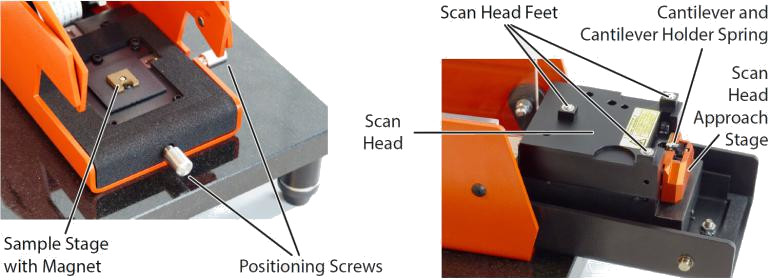
\includegraphics[width=0.7\textwidth]{naioafm2}
\caption{Different parts of the scan head of the NaioAFM instrument \cite{NaioAFM}.}
\label{fig:naioafm}
\end{figure}

\begin{figure}[hbt]
\centering
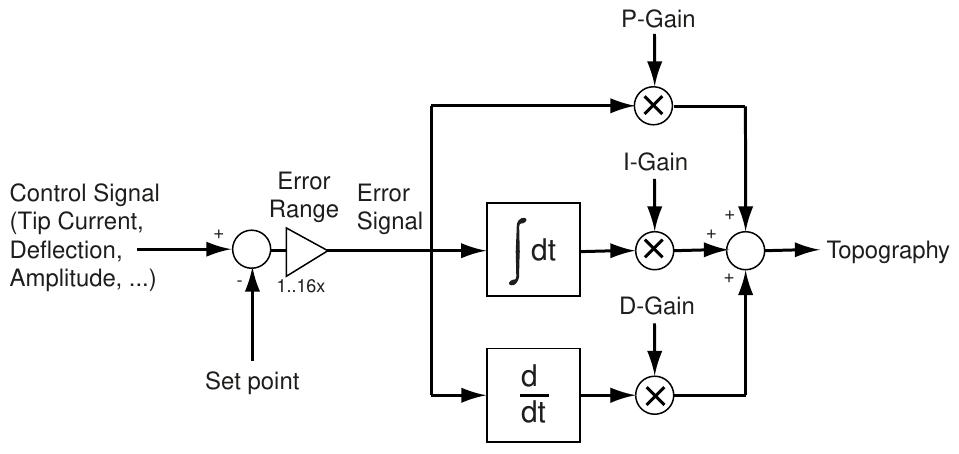
\includegraphics[width=0.6\textwidth]{Feedback_NaioAFM}
\caption{Diagram of the Z-controller of the NaioAFM from the instrument's manual.}
\label{fig:feedback_z-controller}
\end{figure}

A diagram of the specific feedback mechanism of the Z-controller that the NaioAFM implements can be seen in Figure \ref{fig:feedback_z-controller}. Using this loop, the NaioAFM continuously tries to keep this feedback parameter constant at its setpoint by adjusting the z-piezo to move the cantilever probe up and down. And the resulting z-piezo movements provide the height information to create the surface topography.

In the static mode, the setpoint is the force (in \si{\nano \N}) affecting the tip. In the tapping mode it is a percentage that represents the threshold in the reduction of the oscillation's amplitude. For example, a setpoint of 60\% means that the Z-controller will move the tip closer to the sample until the vibration amplitude has decreased to 60\% of the vibration amplitude when it is far away from the sample.

According to the owner's manual from Nanosurf, the integral gain is the most important gain value and can have a dramatic effect on the image quality. The proportional gain might provide slight improvement only after the integral gain has been optimized. And the derivative gain is mainly for samples with tall edges.

Regarding the tips, we use two different types, both made of Silicon nitride (Si$_3$N$_4$): \texttt{PPP-CONTR-20} for the static mode and \texttt{Tap190Al-G} for tapping mode. Static mode cantilever seemed for us not to fit well in the holder.

\subsection{Calibration sample}

Thes sample used to test and optimize parameters of the NaioAFM was the Calibration Standard \texttt{HS-100MG}, whcih has six different surfaces (see Figure \ref{fig:HS-100MG}).

\begin{figure}[H]
\centering
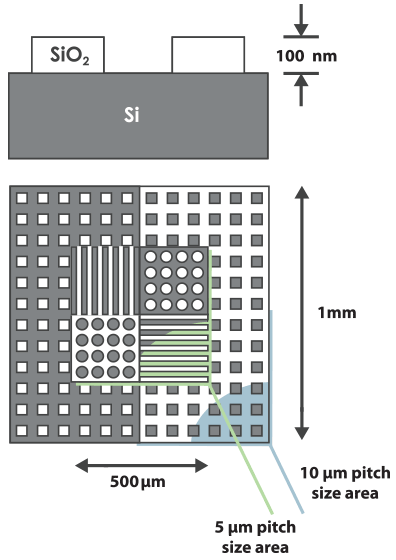
\includegraphics[width=0.34\textwidth]{HS-100MG}
\caption{Dimensions of the calibration sample HS-100MG.}
\label{fig:HS-100MG}
\end{figure}

\subsection{Gwyddion}

NaioAFM saves the data obtained by the samples in \texttt{.nid} files. These files contain 3-dimensional data of the sample: to every point in the (x,y) plane there is an associated height. The height is shown in 2-dimensional heatmaps using a gray colormap. The lighter the gray, the higher the z point is (see Figure \ref{fig:heatmap_rawdata}.)

It is possible to partially correct the noisy parts of the pictures manually or by means of some automatic tools. The data can be levelled by subtracting the mean plane; this corrects situations like the one shown in Figure~\ref{fig:artifacts_processing_1}. Secondly, it is possible to align the raws horizontally or vertically evaluating the median of the differences between them (the error that this tool is able to correct is shown in Figure~\ref{fig:artifacts_processing_2}). A third tool often used is the correction of the horizontal scars.

Moreover, the software allow us to model the colour scale by selecting the height range (Figure~\ref{fig:scale_selection}) and to set the 0 of the z-axis.

\begin{figure}[ht]
\centering
\begin{subfigure}[b]{0.45\textwidth}
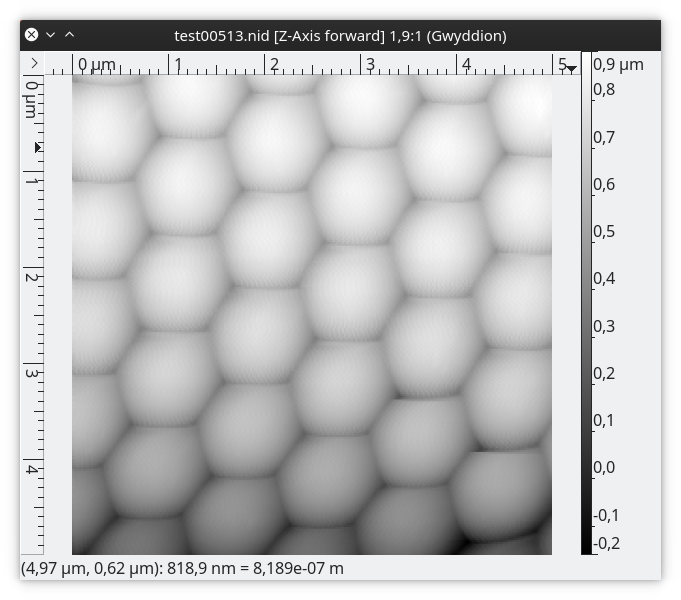
\includegraphics[width=\textwidth]{heatmap_rawdata}
\caption{Raw heatmap shown in Gwyddion after importing raw data from NaioAFM without any processing.}
\label{fig:heatmap_rawdata}
\end{subfigure}
\begin{subfigure}[b]{0.45\textwidth}
\centering
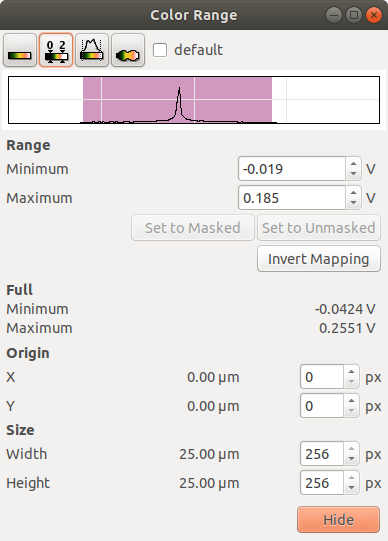
\includegraphics[width=0.7\textwidth]{scale_selection}
\caption{Selection of the height interval.}
\label{fig:scale_selection}
\end{subfigure}
\caption{Some screenshots of Gwyddion.}
\label{fig:gwyddion}
\end{figure}

Finally, Gwyddion allows us to improve the aesthetics of the images, making them more intuitive. First of all, we can select the colour scale which labels the height of the picture. Secondly, the software is able to generate a 3-dimensional pictures of the sample, as we will see in the following section.

\newpage
\section{Results and discussion}
In this section we will showed the images we obtained for the calibration sample and for the three different samples using both modes. Comparison tables (\ref{table:comparison} and \ref{table:comparison2}) between modes can be found at the end of the section.

\subsection{Static mode}
\subsubsection{Calibration}
First, we used the calibration sample with a known surface in order to test the tip and the software used to obtain our data. 

We fixed the sample in the centre of the AFM and used the camera installed inside our Nanosurf NaioAFM equipment to place the tip in the different surfaces (shown in Figure~\ref{fig:cal_sam}).

\begin{figure}[H]
\centering
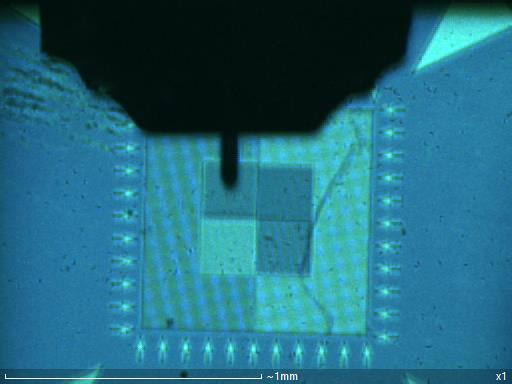
\includegraphics[scale=0.4]{calibration_sample}
\caption{Calibration sample view from the camera installed in Nanosurf NaioAFM}
\label{fig:cal_sam}
\end{figure}

Once we had chosen the surface which we wanted to analyse, by using the software, we moved the tip as close as possible to the sample, without making them contact. Then, using the \emph{approach mode}, we brought the tip in contact with the surface. This mode uses the setpoint and the feedback mechanism to very slowly put the tip in contact minimizing the risk of breaking the tip.

The parameter we tried to optimize was the setpoint. In the software, the setpoint is express in \si{\nano N} and it is calculated by multiplying the deflection with the spring constant of the selected cantilever, which we had to choose before doing anything. A setpoint too high may damage the tip. We did eight measurements with setpoints from \SI{2}{\nano N} to \SI{20}{\nano N}. There were not significant differences (see Appendix \ref{app:static_mode_setpoint}) so we decided to use the intermediate value of \SI{10}{\nano\m} for the rest of the measurements. We did not have time to optimize the PID values so we used the default and suggested ones: $\text{I-Gain}=1000$ and $\text{P-Gain}=1000$.

In the Figure \ref{fig:static_calibration_grid}, three different shapes captured from our calibration sample with these parameters are shown. The obtained height of the patterns was between \SI{114}{\nano m} and \SI{180}{\nano n} (see Table \ref{table:comparison}) after some processing using the read value tool (see screenshot \ref{fig:read_tool}) for some random positions of the pictures. These values were higher than those provided by the calibration sample. We could have forced Gwyddion to have \SI{100}{\nano m} as the height for the features, but additional image processing artifact would have been introduced.

Is possible to observe the x-scale on the top of the pictures, the y-scale on the left and the height colour scale on the right.

\begin{figure}[H]
\centering
\begin{subfigure}[b]{0.45\textwidth}
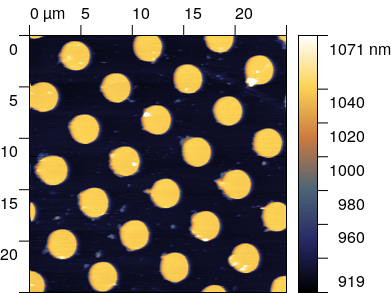
\includegraphics[width=\textwidth]{sm_points}
\caption{Points surface}
\end{subfigure}
\begin{subfigure}[b]{0.45\textwidth}
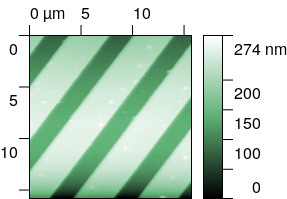
\includegraphics[width=\textwidth]{sm_raws}
\caption{Raws surface}
\end{subfigure}\\\vspace{.2cm}
\begin{subfigure}[b]{0.45\textwidth}
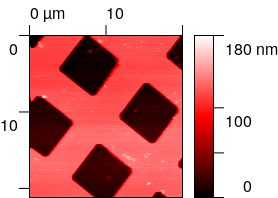
\includegraphics[width=\textwidth]{sm_squares}
\caption{Squares surface}
\end{subfigure}
\begin{subfigure}[b]{0.45\textwidth}
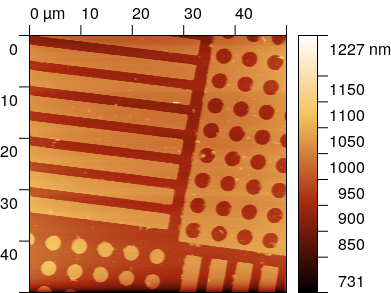
\includegraphics[width=\textwidth]{sm_border}
\caption{Middle of the sample between different patterns}
\end{subfigure}
\caption{Some pictures of different parts of the calibration sample (see Figure \ref{fig:HS-100MG}).}
\label{fig:static_calibration_grid}
\end{figure}

\begin{figure}[H]
\centering
\begin{subfigure}[b]{0.45\textwidth}
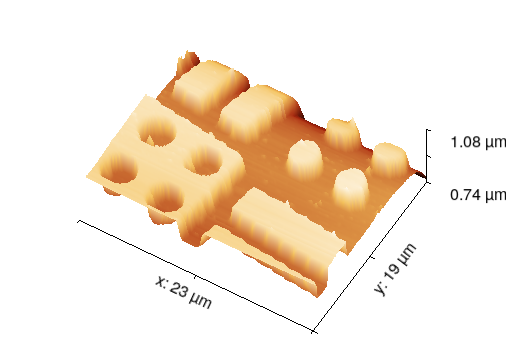
\includegraphics[scale=0.47]{sm_border_3D}
\caption{}
\label{fig: cal sam border}
\end{subfigure}
\begin{subfigure}[b]{0.45\textwidth}
\centering
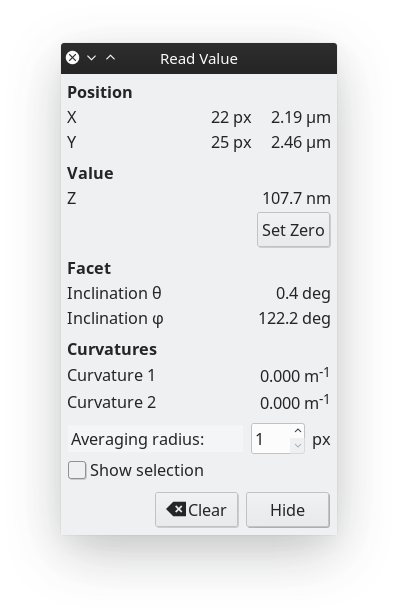
\includegraphics[width=0.6\textwidth]{static_mode_read_value_height}
\caption{}
\label{fig:read_tool}
\end{subfigure}
\caption{(a) A 3D plot of the calibration sample at the middle where pattern changes, and (b) the read tool used to obtain the height value.}
\label{fig:3d_and_read_value}
\end{figure}

The previous pictures have been processed using Gwyddion software. First of all we used some masks to eliminate automatically some imperfections, as for instance orizontal tears caused by abrupt movements of the tip. Secondly, we adjusted the high scale in which the shade of colors had to variate. Finally, we chose four different colour scales in order to better distinguish the four pictures.

We can notice that the lenght scale of the pictures on the top and on the sides. Additionally, a 3D image from the data taken in the middle of the sample can be seen in Figure \ref{fig: cal sam border}.

\subsubsection{Sample 1}
The first sample was labelled as \texttt{Cr \SI{2}{\nano m}, Al \SI{20}{\nano m}}. We were able to make one measurement in the dark part of the sample before having some issues doing the approach (Figures \ref{fig:sample1_first_tip} and \ref{fig:sample1_first_tip2}). We decided to change the tip but the next measurement (Figures \ref{fig:sample1_second_tip} and \ref{fig:sample1_second_tip2}) suffered from an distorsion, an artifact probably due to a certain angle between the tip and the sample's surface as shown previoulsy in Figure \ref{fig:artifacts_scanner_2}. We found quite difficult to fit the static tip in the NaioAFM.

\begin{figure}[H]
\centering
\begin{subfigure}[b]{0.45\textwidth}
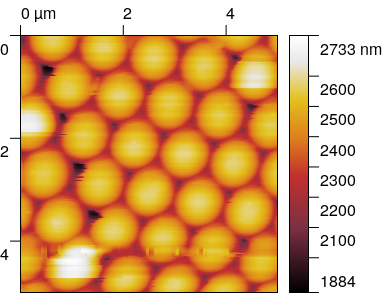
\includegraphics[width=\textwidth]{sm_sample1}
\caption{}
\label{fig:sample1_first_tip}
\end{subfigure}
\begin{subfigure}[b]{0.45\textwidth}
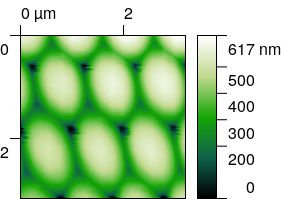
\includegraphics[width=\textwidth]{sm_sample1_dir2}
\caption{}
\label{fig:sample1_second_tip}
\end{subfigure}\\\vspace{.2cm}
\begin{subfigure}[b]{0.45\textwidth}
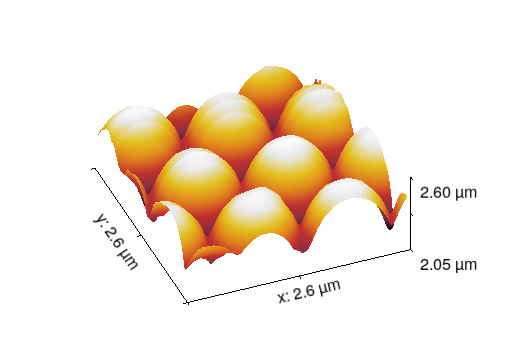
\includegraphics[width=\textwidth]{sm_sample1_3D}
\caption{}
\label{fig:sample1_first_tip2}
\end{subfigure}
\begin{subfigure}[b]{0.45\textwidth}
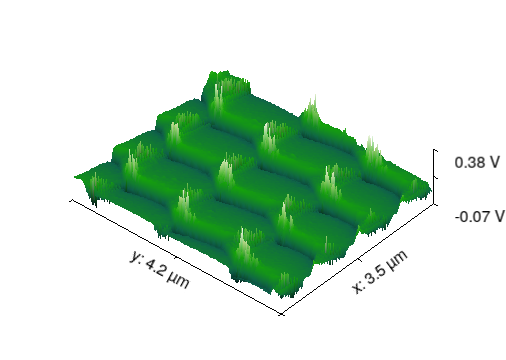
\includegraphics[width=\textwidth]{sm_sample1_dir2_3D}
\caption{}
\label{fig:sample1_second_tip2}
\end{subfigure}
\caption{2D surface images, (a) and (b), and 3D images, (c) and (d), of sample 1. A scanner artifact is very clear in the second measurement (b) and (d) after changing the tip in the AFM.}
\label{fig:sample1_static_general}
\end{figure}

We can see from the two measurements that we have some kind of honeycomb structure with spheres of height $\sim\SI{0.5}{\micro m}$. Also, the distance between the centers of these features for the image without the artifact were $\sim\SI{1}{\micro\m}$ (see Table \ref{table:comparison2}).

\newpage
\subsubsection{Sample 3}
We did not have enough time to measure sample 3 in the static mode. Results for this sample are shown in the tapping mode section \ref{sec:sample3_tapping}.

\subsubsection{Sample 2}
The second sample contained gold particles in silicon dioxide. We can see from Figure \ref{fig:sample_3_static} that the surface of this material was scratched and with some imperfections.

We noticed two distinguishable parts in the sample: light and dark green. We first decide to measure in the dark green areas and in the frontier between dark and green as shown in Figure \ref{fig:sample_3_static}.

\begin{figure}[H]
\centering
\begin{subfigure}[b]{0.4\textwidth}
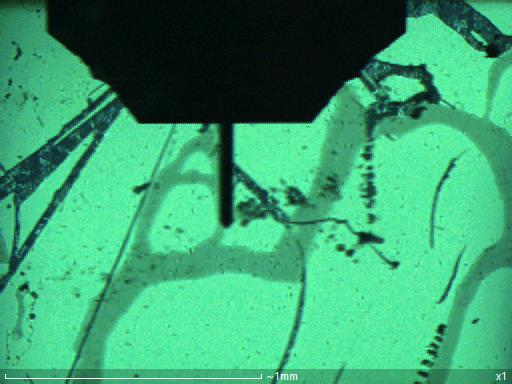
\includegraphics[width=\textwidth]{sm_sample2_set.JPG}
\caption{}
\label{fig:sample_3_static}
\end{subfigure}\\
\begin{subfigure}[b]{0.45\textwidth}
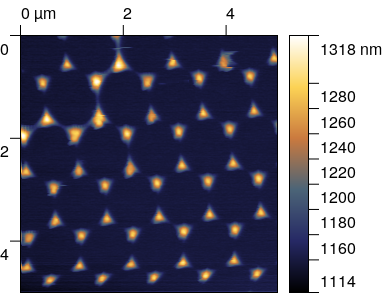
\includegraphics[width=\textwidth]{sm_sample2}
\caption{}
\end{subfigure}
\begin{subfigure}[b]{0.45\textwidth}
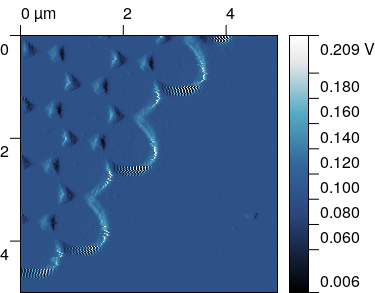
\includegraphics[width=\textwidth]{sm_sample2_border}
\caption{}
\end{subfigure}\\\vspace{.2cm}
\begin{subfigure}[b]{0.45\textwidth}
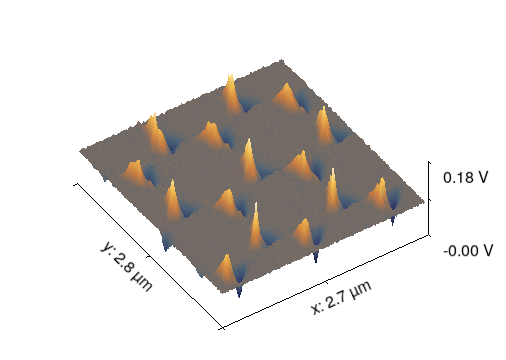
\includegraphics[width=\textwidth]{sm_sample2_3D}
\caption{}
\end{subfigure}
\begin{subfigure}[b]{0.45\textwidth}
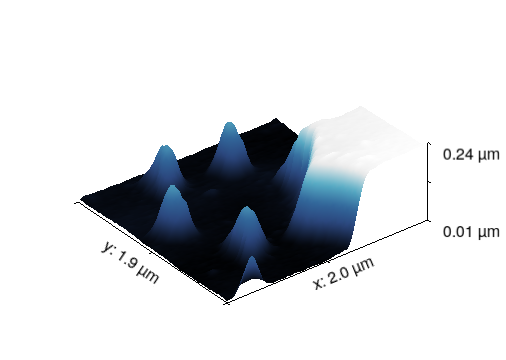
\includegraphics[width=\textwidth]{sm_sample2_border_3D}
\caption{}
\end{subfigure}
\caption{Images obtained in the dark green area and in the frontier for the sample 2. In (a) a screenshot from the NaioAFM camera of the location of the tip when we did the measurement. 2D surface images, (b) and (c), and 3D images, (d) and (e), of sample 2. (b) and (d) were obtained in the dark green area (see Figure \ref{fig:sample_3_static}) of the sample, and (c) and (e) in the frontier between the light and dark green area.}
\end{figure}

We can observe that the plot reminds a set of stars. Moreover, we can see that the surface outside this plot is flat compared to the edges of the star. This triangle patterns may be an artifact due to the fact that the tip is as big as the feature in the surface we are trying to observe. We think that this corresponds to the golden particles.

Then we decide to measure only in the lighter part. We took only one measurement in the center of the light green part as shown in Figure \ref{fig:sample3_light_green_cam}. In this measurement (see Figure \ref{fig:sample3_light_green}) we can notice a hilly surface, but without the interesting pattern found in the dark areas of the sample.

\begin{figure}[H]
\centering
\begin{subfigure}[b]{0.4\textwidth}
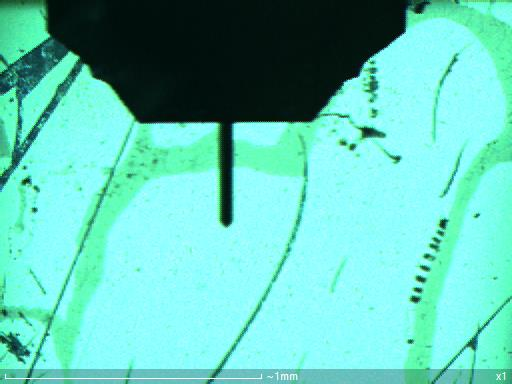
\includegraphics[width=\textwidth]{sm_sample3_set}
\caption{}
\label{fig:sample3_light_green_cam}
\end{subfigure}\\
\begin{subfigure}[b]{0.45\textwidth}
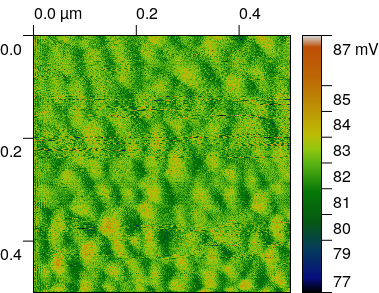
\includegraphics[width=\textwidth]{sm_sample3}
\caption{}
\end{subfigure}
\begin{subfigure}[b]{0.45\textwidth}
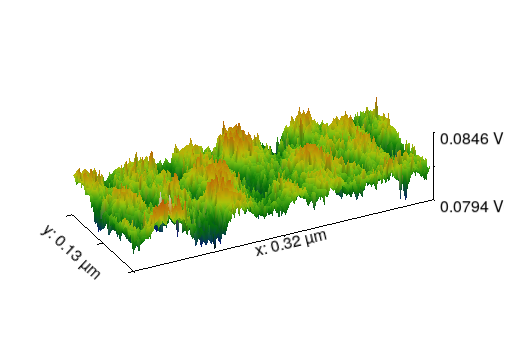
\includegraphics[width=\textwidth]{sm_sample3_3D_improved}
\caption{}
\end{subfigure}
\caption{Images obtained in the light green area of the sample 2. In (a) a screenshot from the NaioAFM camera of the location of the tip when we did the measurement. In (b) and (c) the 2D obtained surface and the 3D generated plot, respectively.}
\label{fig:sample3_light_green}
\end{figure}

\newpage
\subsection{Tapping mode}
After changing the tip, the first thing we had to do was find the frequency of the cantilever. This was done automatically by the NaioAFM software with the \emph{Frequency Sweep} procedure.

\subsubsection{Calibration}
Once again, the first step was the measurement of the calibration sample. For the default gain values ($\text{P-Gain}=1000$ and $\text{I-Gain}=1000$), we did several measurements with different values of the setpoint.

With the calibration grid we tried setpoints of 45\%, 50\%, 65\% and 75\%. For values larger than 65\% the z-controller was not able to follow the surface of the sample (see Appendix \ref{app:tapping_mode_setpoint}). We fixed the setpoint at 45\% for the rest of the measurements and then we tried to optimize the PID values. We only noticed differences by varying the I-Gain value (see Appendix \ref{app:tapping_mode_Igain}). Best result was obtained with $\text{I-Gain}=1500$. We did not observed significant differences changing P-Gain with setpoint and I-Gain values fixed at 45\% and 1500, respectively.


\begin{figure}[H]
\centering
\begin{subfigure}[b]{0.42\textwidth}
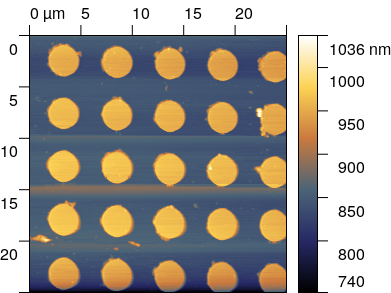
\includegraphics[width=\textwidth]{tm_points}
\caption{Points surface}
\label{fig:}
\end{subfigure}
\begin{subfigure}[b]{0.42\textwidth}
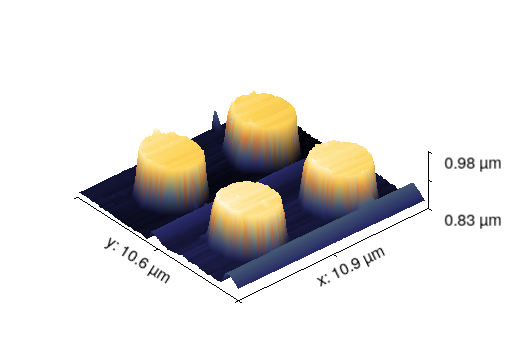
\includegraphics[width=\textwidth]{tm_points_3D}
\caption{Points surface, 3D plot}
\label{fig:sm_raws}
\end{subfigure}\\\vspace{.2cm}
\begin{subfigure}[b]{0.42\textwidth}
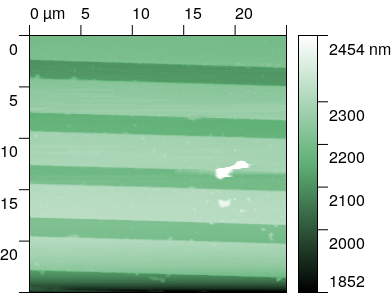
\includegraphics[width=\textwidth]{tm_raws}
\caption{Raws surface}
\label{fig:}
\end{subfigure}
\begin{subfigure}[b]{0.42\textwidth}
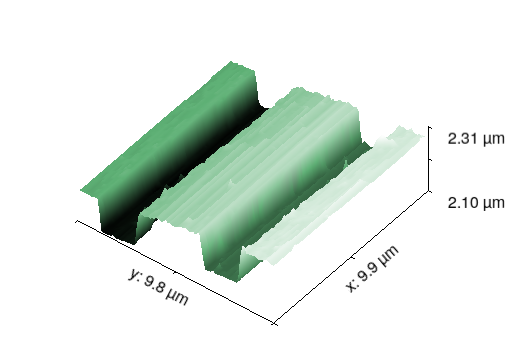
\includegraphics[width=\textwidth]{tm_raws_3D}
\caption{Raws surface, 3D plot}
\label{fig:}
\end{subfigure}\\\vspace{.2cm}
\begin{subfigure}[b]{0.42\textwidth}
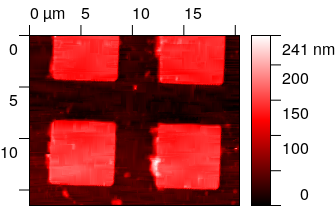
\includegraphics[width=\textwidth]{tm_squares}
\caption{Squares surface}
\label{fig:}
\end{subfigure}
\begin{subfigure}[b]{0.42\textwidth}
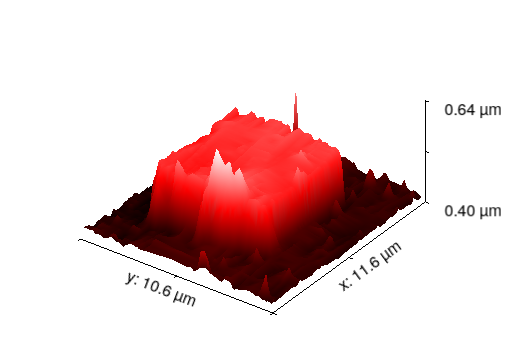
\includegraphics[width=\textwidth]{tm_squares_3D}
\caption{Squares surface, 3D plot}
\label{fig:sm_border}
\end{subfigure}
\caption{Some pictures of the calibration sample using the tapping mode.}\label{fig:: tm cal}
\end{figure}
As we can see, the data obtained is in agreement with the ones picked up with static mode. The height of the plots are in both modes around \SI{0.16}{\micro\m}. The corners are a bit less rounded in this mode, we can notice this fact comparing Figure~\ref{fig:3d_and_read_value} with the 3-dimensional plot in Figure~\ref{fig:: tm cal}.

\subsubsection{Sample 1}
In Figure \ref{fig:tapping_sample1} we can see the picture resulting from the data got about the first sample.

\begin{figure}[H]
\centering
\begin{subfigure}[b]{0.45\textwidth}
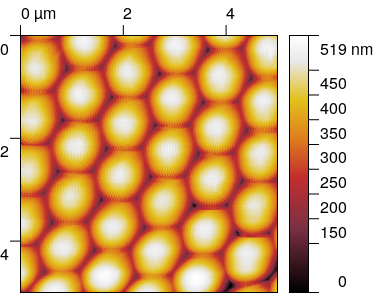
\includegraphics[width=\textwidth]{tm_sample1}
\caption{}
\end{subfigure}
\begin{subfigure}[b]{0.45\textwidth}
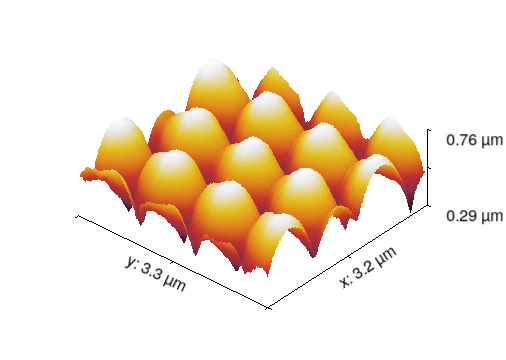
\includegraphics[width=\textwidth]{tm_sample1_3D}
\caption{}
\end{subfigure}
\caption{Images obtained for the sample 1 in tapping mode. In (a) the 2D obtained surface and in (c) the 3D generated plot.}
\label{fig:tapping_sample1}
\end{figure}

The obtained patterns is the same we obtained in the static mode. However, the obtained height is not perfectly in agreement. With the tapping mode we measured \SI{0.43}{\micro\m} while with the static mode we obtained \SI{0.56}{\micro\m} (see Table \ref{table:comparison2}).

\subsubsection{Sample 2}

In Figure \ref{fig:tapping_sample2} we show the obtained images for the second sample.

\begin{figure}[H]
\centering
\begin{subfigure}[b]{0.45\textwidth}
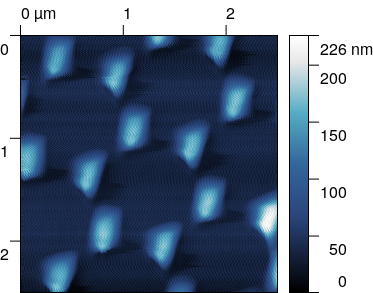
\includegraphics[width=\textwidth]{tm_sample2}
\caption{}
\end{subfigure}
\begin{subfigure}[b]{0.45\textwidth}
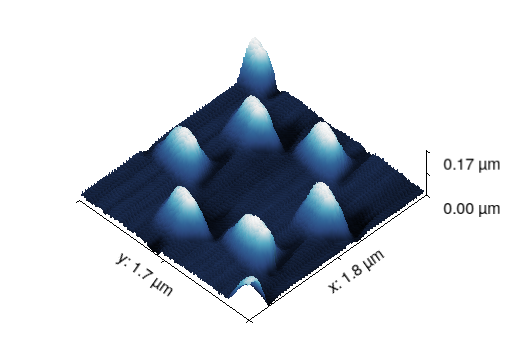
\includegraphics[width=\textwidth]{tm_sample2_3D}
\caption{}
\end{subfigure}
\caption{Images obtained for the sample 2 in tapping mode. In (a) the 2D obtained surface and in (c) the 3D generated plot.}
\label{fig:tapping_sample2}
\end{figure}

Again, we were able to replicate the obtained patter using the static mode, which reminds us of a set of stars. Besides, in this case, the obtained height with both modes were very similar, \SI{0.19}{\micro\m} in the case of static mode, and \SI{0.17}{\micro\m} in the tapping mode (see Table \ref{table:comparison}).

\subsubsection{Sample 3}\label{sec:sample3_tapping}

Finally, in Figure \ref{fig:tapping_sample3} we can see the pictures obtained for the third sample.

\begin{figure}[H]
\centering
\begin{subfigure}[b]{0.45\textwidth}
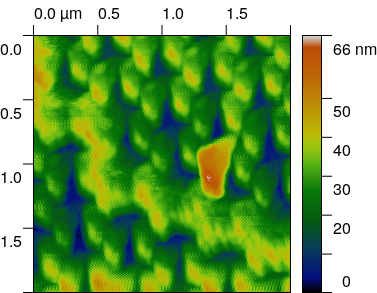
\includegraphics[width=\textwidth]{tm_sample3}
\caption{Sample 3 in tapping mode}
\label{fig:}
\end{subfigure}
\begin{subfigure}[b]{0.45\textwidth}
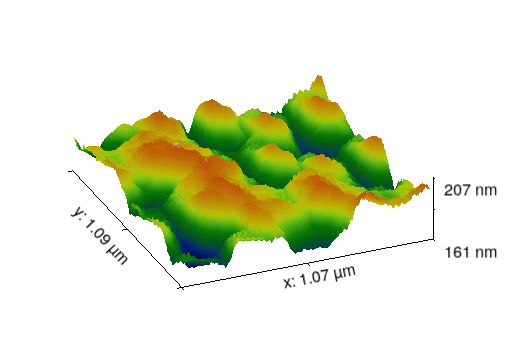
\includegraphics[width=\textwidth]{tm_sample3_3D}
\caption{}
\end{subfigure}
\caption{Images obtained for the sample 3 in tapping mode. In (a) the 2D obtained surface and in (c) the 3D generated plot.}
\label{fig:tapping_sample3}
\end{figure}

In this case we can state that the plot of the material is not very regular.

At this point we attach a table of the maximum heights measured thanks to Gwyddion (as far as the 3 samples are concerned we will write the maximum height).

\begin{table}[H]
\centering
\begin{tabular}{l c c}
\toprule
& Static mode (\si{\nano\m}) & Tapping mode (\si{\nano\m})\\
\midrule
Points   & 180 & 180 \\
Raws     & 121 & 150 \\
Squares  & 114 & 128 \\
Sample 1 & 560 & 430 \\
Sample 2 & 190 & 170 \\
Sample 3 & -- & 44 \\
\bottomrule
\end{tabular}
\caption{Table comparing the heights obtained both in static mode and in tapping mode for different parts of the calibration sample and for the features observed in the three samples.}
\label{table:comparison}
\end{table}

Comparing the table with the pictures, we can see that it is not always clear from the images to estimate the height. Actually, even the data reported here are not very precise because of the peaks and hills; it is not always clear from which two points to measure the z-distance because the surfaces are often not regular.

We also show the distance between the centers of the cells measured from the data got in both the modes. As we can see, the values are in good agreement between them.

\begin{table}[H]
\centering
\begin{tabular}{l c c}
\toprule
Mode & Sample 1 (\si{\micro\m}) & Sample 2 (\si{\micro\m}) \\
\midrule
Static & 1.018 & 1.126 \\
Tapping & 1.040 & 1.060 \\
\bottomrule
\end{tabular}
\caption{Table comparing the distances between centers of the features.}
\label{table:comparison2}
\end{table}

\newpage
\section{Conclusions}
An overview of the theory of AFM, two of its operation modes, the feedback mechanism and AFM artifacts was presented at the beginning of the report.

In contrast to our initial thought, we observed that in static mode the setpoint value was not relevant in the range from \SI{2}{\nano\N} to \SI{20}{\nano\N}. Maybe significant differences can be noticed for larger values, but we did not try to avoid breaking the tip. Optimized PID values for static mode were not found due to lack of time (we had to change the tip in two occasions). On the contrary, in tapping mode we did find the upper limit of 65\% to the setpoint, at which for larger values the z-controller was not able to follow the surface of the sample. Optimized I-Gain value was found at 1500, and P-Gain was not relevant in our setup after fixing the previous two parameters. In general, we found working in tapping mode easier, perhaps due to the use of an inappropriate tip in static mode, which made the process of placing it in the NaioAFM very difficult.

Larger value than those provided in the calibration sample were measured in both static and tapping mode. Two interesting patterns were observed in the first and second sample. We were able to observed them in the two modes and obtain similar values for the height of the features, as well as for the separation distances between its centers. No pattern but an irregular surface was found in third sample.

\nocite{*}
\vfill
\bibliographystyle{unsrt}
\bibliography{references}

\newpage
\begin{appendices}
\section{Different setpoints in static mode}\label{app:static_mode_setpoint}

\begin{figure}[H]
\centering
\begin{subfigure}[b]{0.48\textwidth}
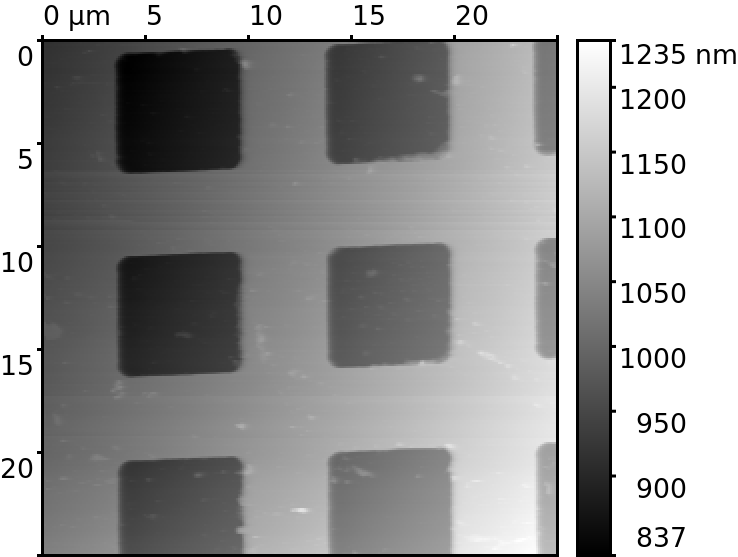
\includegraphics[width=\textwidth]{static_mode_setpoint_2}
\caption{\SI{2}{\nano\N}}
\end{subfigure}
\begin{subfigure}[b]{0.48\textwidth}
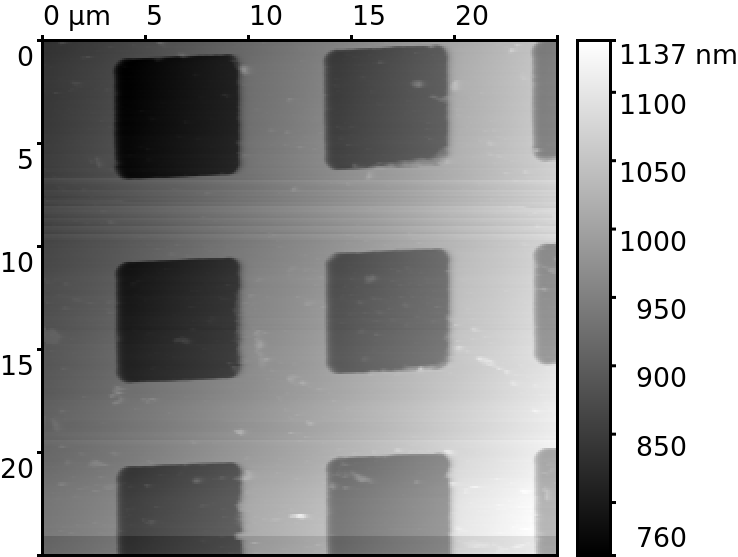
\includegraphics[width=\textwidth]{static_mode_setpoint_5}
\caption{\SI{5}{\nano\N}}
\end{subfigure}\\\vspace{.2cm}
\begin{subfigure}[b]{0.48\textwidth}
\includegraphics[width=\textwidth]{static_mode_setpoint_10}
\caption{\SI{10}{\nano\N}}
\end{subfigure}
\begin{subfigure}[b]{0.48\textwidth}
\includegraphics[width=\textwidth]{static_mode_setpoint_20}
\caption{\SI{20}{\nano\N}}
\end{subfigure}
\caption{Raw images obtained in static mode using the calibration sample with different values of the setpoint keeping the same values for the PID gains. Row artifacts occur randomly independently of the setpoint used and probably due to the scanner. Slower measurements would have given better images but requiring a lot more time.}
\end{figure}

\section{Different setpoints in tapping mode}\label{app:tapping_mode_setpoint}

\begin{figure}[H]
\centering
\begin{subfigure}[b]{0.48\textwidth}
\includegraphics[width=\textwidth]{tapping_mode_setpoint_45}
\caption{45\%}
\end{subfigure}
\begin{subfigure}[b]{0.48\textwidth}
\includegraphics[width=\textwidth]{tapping_mode_setpoint_50}
\caption{50\%}
\end{subfigure}\\\vspace{.2cm}
\begin{subfigure}[b]{0.48\textwidth}
\includegraphics[width=\textwidth]{tapping_mode_setpoint_65}
\caption{65\%}
\end{subfigure}
\caption{Raw images obtained in tapping mode using the calibration sample with different values of the setpoint keeping the same values for the PID gains. For the value of 65\% it was already difficult to see the pattern. For larger values, the z-controller was not able to follow the surface of the sample.}
\end{figure}

\section{Different I-Gain values in tapping mode}\label{app:tapping_mode_Igain}

\begin{figure}[H]
\centering
\begin{subfigure}[b]{0.48\textwidth}
\includegraphics[width=\textwidth]{tapping_mode_Igain_500}
\caption{$\text{I-Gain}=500$}
\end{subfigure}
\begin{subfigure}[b]{0.48\textwidth}
\includegraphics[width=\textwidth]{tapping_mode_Igain_1500}
\caption{$\text{I-Gain}=1500$}
\end{subfigure}\\\vspace{.2cm}
\begin{subfigure}[b]{0.48\textwidth}
\includegraphics[width=\textwidth]{tapping_mode_Igain_2000}
\caption{$\text{I-Gain}=2000$}
\end{subfigure}
\caption{Raw images obtained in tapping mode using the calibration sample with different values of the I-Gain value keeping the setpoint constant at 45\%. Image obtained with $I=1500$ was the best result.}
\end{figure}

\end{appendices}
\end{document}